\documentclass[t, notes, xcolor=table]{beamer}

\usepackage{wrapfig}
\usepackage{float}
% For tabs in verbatim
\usepackage{fancyvrb}

% Adjust position of the image
\usepackage[export]{adjustbox}

% set fonts
\usefonttheme{professionalfonts} % using non standard fonts for beamer
\usepackage{txfonts,mathptmx}

% set indend spacing for first and second level indentation
\setlength{\leftmargini}{0.5cm}
\setlength{\leftmarginii}{0.5cm}
\setlength{\leftmarginiii}{0.5cm}

% Set circles for bullets 
\setbeamertemplate{itemize items}[circle]

% colors
\usepackage{xcolor}

% multiple columns
\usepackage{multicol}

% todo lists
\usepackage{pifont}
\usepackage{amssymb}

% increase space between text and frame name
\addtobeamertemplate{frametitle}{}{\vspace{0.5em}}

%Information to be included in the title page:
\title{Coding RTL for Synthesis}
\author{Nikola Petrovic}
\institute{University of Belgrade, School of Electrical Engineering}
\date{2022}



\begin{document}

\frame{\titlepage}

%%%%%%%%%%%%%%%%%%%%%%%%%%%%%%%%%%%%%%%%%%%%%%%%%%%%%%%%%%%%
\begin{frame}
\frametitle{Module Objective}
In this module we will code design behaviour for logic synthesis.
\newline

\textbf{Topics:}
\begin{itemize}
\item Modeling combinational logic
\item Modeling sequential logic
\item Modeling latch logic
\item Modeling three-state logic
\item Using synthesis attributes
\end{itemize}
\end{frame}
\note{
\scriptsize{
Our objective is to code design behaviours for logic synthesis.
\newline

To do that, we need to know about:
\begin{itemize}
\item Modeling combinational logic
\item Modeling sequential logic
\item Modeling latch logic
\item Modeling three-state logic
\item Using synthesis attributes
\end{itemize}

}
}

%%%%%%%%%%%%%%%%%%%%%%%%%%%%%%%%%%%%%%%%%%%%%%%%%%%%%%%%%%%%
\begin{frame}
\frametitle{Modeling Combinational Logic}
Combinational Logic: Output is at all times a combinational function solely of the inputs.
\scriptsize{
\begin{multicols}{2}
\begin{itemize}
\item As a \textbf{net declaration} assignment
\item As a \textbf{continuous} assignment
\item As an \textbf{always} statement
\end{itemize}
\vfill
\columnbreak
\begin{figure}
    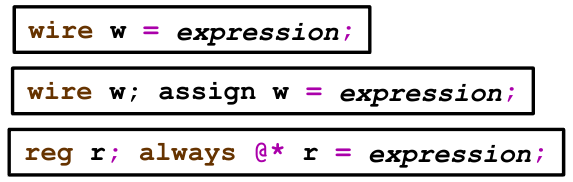
\includegraphics[width=0.45\textwidth]{img/13_seq_1.png}
\end{figure}
\end{multicols}
\begin{itemize}
\item The event list must not contain a posedge or negedge event.
\begin{itemize}
	\scriptsize{
	\item[$-$] Include all procedure inputs to avoid mismatch between pre-synthesis and post-synthesis designs.	
	}
\end{itemize}
\item Assignments must be blocking, they are sufficient and simulate more efficiently.
\end{itemize}
}
\begin{figure}
    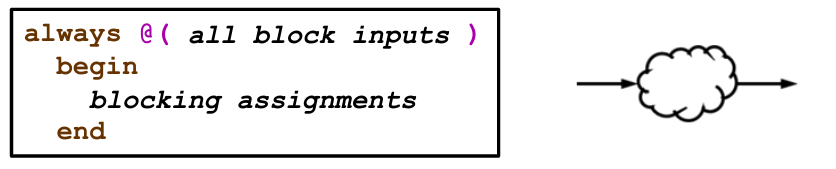
\includegraphics[width=0.75\textwidth]{img/13_seq_2.png}
\end{figure}
\end{frame}
\note{
\tiny{
We can model combinational logic with a net declaration assignment or a continuous assignment or an \textit{always} statements.
\newline

When using an \textit{always} statement, the single event list must not contain a \textit{posedge} or \textit{negedge} event. The event list does not otherwise affect the synthesis results, but to avoid incorrect RTL simulation results, we should include in the event list all inputs to the procedure. The easiest way to ensure this is to use the Verilog 2001 wild-card event control (@*).
\newline

We must not in an \textit{always} statement assign a variable using both a blocking and a non-blocking assignment The blocking assignment is sufficient for a description of combinational logic and simulates more efficiently than the non-blocking assignment.
\newline

\textbf{From IEEE Std. 1364.1-2002} \textit{Section 5.1}:

Combinational logic shall be modeled using a continuous assignment or a net declaration assignment or an
always statement.
\newline

When using an always statement, the event list shall not contain an edge event (posedge or negedge). The
event list does not affect the synthesized netlist. However, it may be necessary to include in the event list all
the variables read in the always statement to avoid mismatches between simulation and synthesized logic.
\newline

A variable assigned in an always statement shall not be assigned using both a blocking assignment (=) and a
nonblocking assignment (\textless=) in the same always statement.
\newline

The event list for a combinational logic model shall not contain the reserved words posedge or negedge. Not
all variables that appear in the right hand side of an assignment are required to appear in the event list. For
example, a variable does not have to appear in the event list of an always statement if it is assigned a value
with a blocking assignment before being used in subsequent expressions within the same always statement.
\newline

The event list may be the implicit event expression list (@(*), @*). 

}
}

%%%%%%%%%%%%%%%%%%%%%%%%%%%%%%%%%%%%%%%%%%%%%%%%%%%%%%%%%%%%
\begin{frame}
\frametitle{Incomplete Event List}
\scriptsize{
\begin{itemize}
\item For simulation, include in the event list all signals that are input to the logic.
\item The "*" wild-card sensitivity list automatically includes all input signals to the logic.
\end{itemize}
}
\begin{figure}
    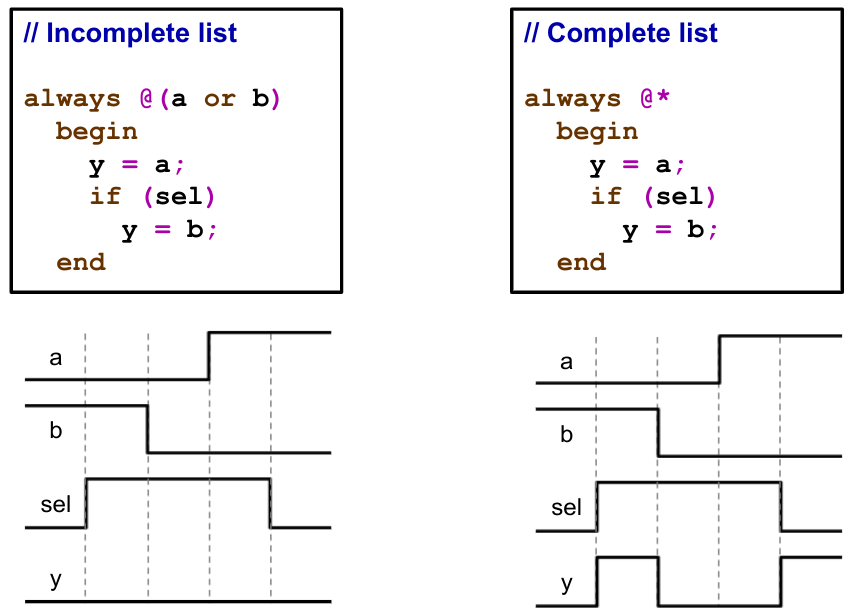
\includegraphics[width=0.65\textwidth]{img/13_event.png}
\end{figure}
\end{frame}
\note{
\scriptsize{
The event list does not affect the synthesis result, but to avoid incorrect RTL simulation results, we should include in the event list all inputs to the procedure. The easiest way to ensure this is to use the Verilog 2001 wildcard event control \textbf{(@*)}.
\newline

This example illustrates the affect of an incomplete sensitivity list.
\begin{itemize}
\item If the event list omits the \textit{sel} signal, the procedure executes upon transitions of only the \textit{a} and \textit{b} inputs - transitions of the \textit{sel} signal have no effect.
\item Debugging problems caused by an incomplete sensitivity list is difficult, so we might want to develop the habit of simply always using the wildcard event control for all combinational procedures.
\end{itemize}

\textbf{From IEEE Std. 1364.1-2002} \textit{Section 5.1}:

"The event list does not affect the synthesized netlist."

}
}

%%%%%%%%%%%%%%%%%%%%%%%%%%%%%%%%%%%%%%%%%%%%%%%%%%%%%%%%%%%%
\begin{frame}
\frametitle{Complete Event List}
\scriptsize{
\begin{multicols}{2}
The event list for a combinational procedure should contain all inputs to the logic.
\begin{figure}
    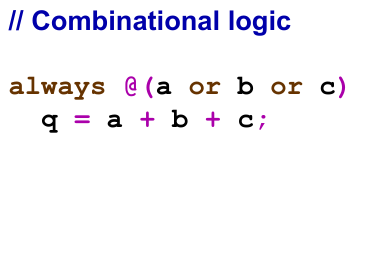
\includegraphics[width=0.35\textwidth,left]{img/13_complete_event_1.png}
\end{figure}
\vfill
\columnbreak
Do not include temporary variables in the sensitivity list.
\begin{figure}
    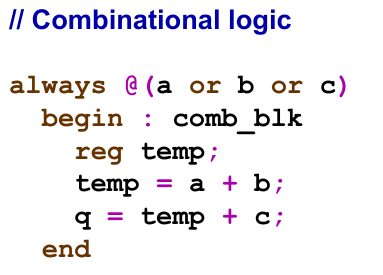
\includegraphics[width=0.35\textwidth,left]{img/13_complete_event_2.png}
\end{figure}
\end{multicols}
}
\end{frame}
\note{
\tiny{
The Verilog language let us place any signals in the sensitivity list and to freely mix blocking and non-blocking assignments anywhere in the procedure. A simulation tool simply executes the procedure as we wrote it, using simulation semantics.
\newline

However, to generate RTL simulation results consistent with those of the post-synthesis netlist, some guidelines exist:
\begin{itemize}
\item All edges of all signals input to combinational logic must be present in the sensitivity list. This is due to the rule that any changes on any input to the logic must have the opportunity to immediately affect the output. \textbf{Do not place temporary variables in the sensitivity list!} A temporary variable is one that the procedure writes only before it reads and that no other procedure uses. It is not an input to the logic.
\item Do not mix blocking and non-blocking assignments to the same variable. Even better, we should use only blocking assignments within procedures that represent purely combinational logic. This is a recommendation to obtain higher simulation performance, as non-blocking assignments are not necessary and simulate more slowly.
\end{itemize}
The synthesis tool requires code that unambiguously states our design intentions. Code meant for the synthesis tool may use only a subset of the Verilog constructs and coding styles.
\begin{itemize}
\item For synthesis, it is an absolute requirement that we don't mix blocking and non-blocking assignments to the same variable!
\item The synthesis standard states that the sensitivity list shall not affect the generation of combinational logic. That means that if the synthesis tool recognizes the block as combinational logic, it will proceed as if we had included all inputs to the logic in the sensitivity list. The synthesis tool may or may not warn us about missing inputs. The generated gates will simulate correctly, but very likely differently that the incorrect RTL simulation.
\end{itemize}

}
}

%%%%%%%%%%%%%%%%%%%%%%%%%%%%%%%%%%%%%%%%%%%%%%%%%%%%%%%%%%%%
\begin{frame}
\frametitle{Incomplete Assignments}
\textbf{Combinational Logic}
\footnotesize{
\begin{itemize}
\item Output is at all times a combinational function solely of the inputs.
\end{itemize}
}
\begin{figure}
    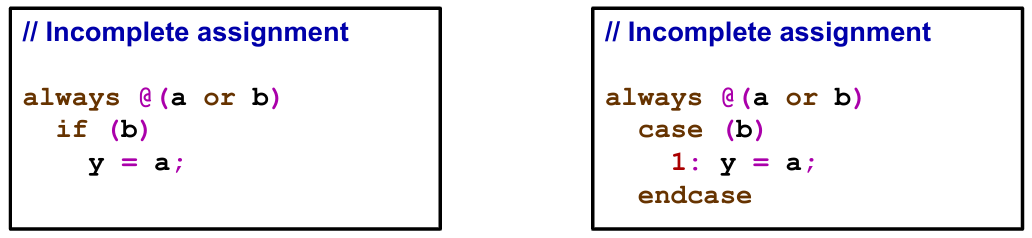
\includegraphics[width=0.95\textwidth]{img/13_incomplete_assign.png}
\end{figure}
\vfill

* What is the value of y when b is 0?
\end{frame}
\note{
\scriptsize{
If an execution path through a combinational procedure exists that does not update the value of some output, then the output variable must retain its previous state. The synthesis tool infers a latch to implement this behaviour. Latch inference is almost always non intended, and we can easily avoid it.
\newline

This example fails to update the \textit{y} output variable when the input \textit{b} is not 1.
\newline

How would you modify this code to ensure inference of purely combinational logic?

}
}

%%%%%%%%%%%%%%%%%%%%%%%%%%%%%%%%%%%%%%%%%%%%%%%%%%%%%%%%%%%%
\begin{frame}
\frametitle{Complete Assignment}
Avoiding latch inference is easy!
\footnotesize{
\begin{itemize}
\item Provide outputs with a value for every combination of inputs.
\item This is most easily done with default assignments.
\end{itemize}
}
\begin{figure}
    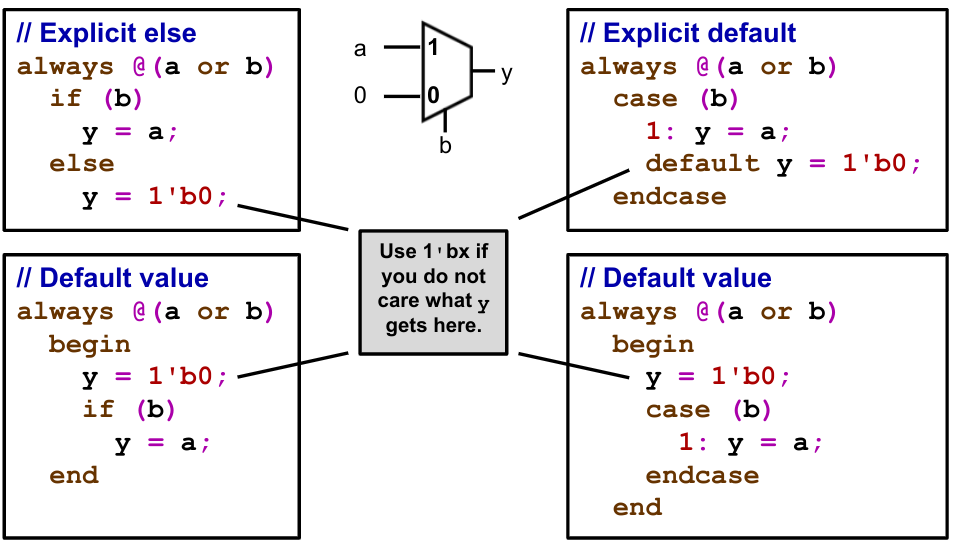
\includegraphics[width=0.75\textwidth]{img/13_complete_assign.png}
\end{figure}
\end{frame}
\note{
\scriptsize{
Here are two methods we can use to prevent latch inference:
\begin{itemize}
\item We can for an \textit{if} statement use an explicit \textit{else} clause and for a \textit{case} statement an explicit default match item.
\item we can provide default values for all procedure outputs at the start of the procedure.
\end{itemize}
Which is the best technique in a real design?
\newline

If we have a procedure with a complex set of conditional assignments, we can easily miss an assignment for one or more of these branches. Making default assignments at the start of the procedure ensures that all procedure outputs have an assignment.
\newline

\textbf{From IEEE Std. 1364.1-2002} \textit{Section 5.5} Support for values x and z:

The value \textbf{x} may be used as a primary on the RHS of an assignment to indicate a don't care value for synthesis.

}
}

%%%%%%%%%%%%%%%%%%%%%%%%%%%%%%%%%%%%%%%%%%%%%%%%%%%%%%%%%%%%
\begin{frame}
\frametitle{Continuous Assignments}
Continuous assignments drive values onto nets.
\newline

Continuous assignments always represent combinational logic.
\begin{itemize}
\item Impossible to not assign a value for some input combination.
\item Output is always a combinational function of current inputs.
\end{itemize}
\vspace{10pt}
\begin{figure}
    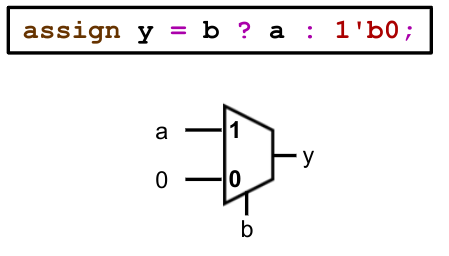
\includegraphics[width=0.45\textwidth]{img/13_cont_assign.png}
\end{figure}
\end{frame}
\note{
\scriptsize{
Continuous assignments and net declaration assignments drive values onto nets. These assignments always represent combinational logic, as it is syntactically impossible to not assign a value for some input combination, thus the output is always a combinational function of the current inputs.

}
}

%%%%%%%%%%%%%%%%%%%%%%%%%%%%%%%%%%%%%%%%%%%%%%%%%%%%%%%%%%%%
\begin{frame}
\frametitle{Modeling Combinational Logic Summary}

\end{frame}
\note{
\scriptsize{


}
}

%%%%%%%%%%%%%%%%%%%%%%%%%%%%%%%%%%%%%%%%%%%%%%%%%%%%%%%%%%%%
\begin{frame}
\frametitle{Module}

\end{frame}
\note{
\scriptsize{


}
}

%%%%%%%%%%%%%%%%%%%%%%%%%%%%%%%%%%%%%%%%%%%%%%%%%%%%%%%%%%%%
\begin{frame}
\frametitle{Module}

\end{frame}
\note{
\scriptsize{


}
}

%%%%%%%%%%%%%%%%%%%%%%%%%%%%%%%%%%%%%%%%%%%%%%%%%%%%%%%%%%%%
\begin{frame}
\frametitle{Module}

\end{frame}
\note{
\scriptsize{


}
}

%%%%%%%%%%%%%%%%%%%%%%%%%%%%%%%%%%%%%%%%%%%%%%%%%%%%%%%%%%%%
\begin{frame}
\frametitle{Module}

\end{frame}
\note{
\scriptsize{


}
}

%%%%%%%%%%%%%%%%%%%%%%%%%%%%%%%%%%%%%%%%%%%%%%%%%%%%%%%%%%%%
\begin{frame}
\frametitle{Module}

\end{frame}
\note{
\scriptsize{


}
}

%%%%%%%%%%%%%%%%%%%%%%%%%%%%%%%%%%%%%%%%%%%%%%%%%%%%%%%%%%%%
\begin{frame}
\frametitle{Module}

\end{frame}
\note{
\scriptsize{


}
}








%%%%%%%%%%%%%%%%%%%%%%%%%%%%%%%%%%%%%%%%%%%%%%%%%%%%%%%%%%%%
\begin{frame}
\frametitle{Test You Understanding - 1}

\begin{itemize}
\item[$\square$] 
\item[$\square$] 
\item[$\square$] 
\item[$\square$] 
\end{itemize}
\end{frame}
\note{

}



\end{document}
